% UFT 中文演讲幻灯片
% Conference presentation template (Chinese)
\documentclass[aspectratio=169]{beamer}

% 中文支持
\usepackage{ctex}
\usepackage{fontspec}
\setmainfont{DejaVu Serif}
\setsansfont{DejaVu Sans}
\setmonofont{DejaVu Sans Mono}

% Theme
\usetheme{Madrid}
\usecolortheme{whale}
\setbeamertemplate{navigation symbols}{}
\setbeamertemplate{footline}[frame number]

% Packages
\usepackage{amsmath,amssymb}
\usepackage{graphicx}
\usepackage{tikz}
\usetikzlibrary{arrows.meta,positioning,calc}

% Colors
\definecolor{darkblue}{RGB}{0,0,139}
\definecolor{darkgreen}{RGB}{0,100,0}
\definecolor{darkred}{RGB}{139,0,0}
\definecolor{uftgold}{RGB}{218,165,32}

% Title info
\title[统一场论]{\textbf{统一场论（UFT）}}
\subtitle{固定4维拓扑—动态谱维\\零自由参数的几何框架}
\author{研究团队}
\institute{UFT研究组}
\date{\today}

\begin{document}

% Title slide
\begin{frame}
\titlepage
\end{frame}

% Outline
\begin{frame}{目录}
\tableofcontents
\end{frame}

% Section 1: The Problem
\section{问题背景}

\begin{frame}{两大理论，一个难题}
\begin{columns}
\column{0.5\textwidth}
\textbf{广义相对论}
\begin{itemize}
    \item 引力和时空几何
    \item 优美而成功
    \item 没有量子效应
\end{itemize}

\vspace{0.5cm}

\textbf{量子力学}
\begin{itemize}
    \item 粒子和力
    \item 极其精确
    \item 没有引力
\end{itemize}

\column{0.5\textwidth}
\begin{block}{冲突}
当两者都重要时：
\begin{itemize}
    \item 黑洞奇点
    \item 大爆炸初始条件
    \item 无穷大和荒谬
\end{itemize}
\end{block}

\begin{alertblock}{目标}
统一引力量子力学的框架
\end{alertblock}
\end{columns}
\end{frame}

\begin{frame}{基础物理中的开放问题}
\begin{enumerate}
    \item \textbf{量子引力}：时空如何从量子原理中产生？
    \item \textbf{暗物质}：维系星系的不可见质量是什么？
    \item \textbf{暗能量}：为什么宇宙在加速膨胀？
    \item \textbf{宇宙学常数}：为什么真空能量这么小却非零？
    \item \textbf{层级问题}：为什么引力比其他力弱这么多？
    \item \textbf{黑洞信息}：落入黑洞的信息会发生什么？
\end{enumerate}

\vspace{0.3cm}
\begin{center}
\textcolor{darkblue}{\textbf{标准模型}：19+自由参数，无引力}\\
\textcolor{darkred}{\textbf{UFT}：0自由参数，包含引力}
\end{center}
\end{frame}

% Section 2: The Core Idea
\section{核心思想}

\begin{frame}{基本原理}
\begin{center}
\Large
\textbf{4维互反空间 $\leftrightarrow$ 10维内空间}\\[0.5cm]
\normalsize
\textit{能量在外空间向内流动}\\
\textit{在内空间向外扩展}\\[0.5cm]
\begin{tikzpicture}[scale=0.8]
    % 4D space
    \draw[thick, blue, fill=blue!10] (0,0) ellipse (2cm and 1cm);
    \node[blue] at (0,-1.5) {\textbf{4维互反空间}};
    \node at (0,0) {\small 外空间};
    \draw[blue, ->] (0.5,0.3) -- (-0.5,0.3);
    \node[blue, above] at (0,0.6) {\small $r \to 0$};
    
    % Arrow
    \draw[thick, red, ->] (2.5,0) -- (4,0);
    \node[red, above] at (3.25,0.2) {\small 对偶};
    
    % 10D space
    \draw[thick, darkgreen, fill=darkgreen!10] (6.5,0) ellipse (2cm and 1cm);
    \node[darkgreen] at (6.5,-1.5) {\textbf{10维内空间}};
    \node at (6.5,0) {\small 内空间};
    \draw[darkgreen, ->] (6,0.3) -- (7,0.3);
    \node[darkgreen, above] at (6.5,0.6) {\small $r_{int} \to \infty$};
\end{tikzpicture}
\end{center}
\end{frame}

\begin{frame}{数学基础：克利福德代数 $Cl(1,9)$}
\begin{columns}
\column{0.5\textwidth}
\textbf{构建模块}
\begin{itemize}
    \item 10个伽马矩阵：$\Gamma^M$，$M = 0,1,\ldots,9$
    \item 度规符号：$(-,+,+,+,+,+,+,+,+,+)$
    \item 32分量旋量
    \item 代数：$\{\Gamma^M, \Gamma^N\} = 2\eta^{MN}$
\end{itemize}

\vspace{0.5cm}

\textbf{关键量}
\begin{itemize}
    \item 扭转场：$\tau_0 = 0.005$
    \item 从信息论推导
    \item 不是拟合——是计算！
\end{itemize}

\column{0.5\textwidth}
\begin{block}{为什么是10维？}
\begin{itemize}
    \item 数学自洽性
    \item 力自然统一
    \item 4维在低能涌现
\end{itemize}
\end{block}

\begin{alertblock}{神奇数字}
\begin{center}
\Large
$\tau_0 = 0.005$
\end{center}
从第一性原理：
\[
\tau_0 = \frac{3d_{out}}{4d_{in}(d_{in}-d_{out})} = \frac{12}{2400}
\]
\end{alertblock}
\end{columns}
\end{frame}

\begin{frame}{谱维：关键洞见}
\begin{center}
\begin{tikzpicture}[scale=0.9]
    % Axes
    \draw[->] (0,0) -- (10,0) node[right] {能量 $E$（对数尺度）};
    \draw[->] (0,0) -- (0,6) node[above] {有效维度 $d_s$};
    
    % Curve
    \draw[thick, blue] (0.5,1) .. controls (2,1.2) and (4,2) .. (6,4);
    \draw[thick, blue] (6,4) .. controls (7.5,5.5) .. (9.5,5.8);
    
    % Labels
    \node[blue, right] at (9.5,5.8) {$d_s = 10$};
    \node[blue, left] at (0.5,1) {$d_s = 4$};
    
    % Critical point
    \draw[dashed, red] (6,0) -- (6,6);
    \node[red, below] at (6,0) {$E_c = 2\times 10^{21}$ GeV};
    
    % Regions
    \node at (3,0.5) {\small 低能：4维物理};
    \node at (8,3) {\small 高能：10维物理};
    
    % Formula
    \node at (5,5.5) {$d_s(E) = 4 + \frac{6}{1+(E/E_c)^2}$};
\end{tikzpicture}
\end{center}

\vspace{0.3cm}
\begin{center}
\textbf{维度不是固定的——它随能量流动！}
\end{center}
\end{frame}

% Section 3: Predictions
\section{粒子物理预测}

\begin{frame}{费米子质量：12个预测，0个拟合}
\begin{center}
\begin{tabular}{lccc}
\toprule
\textbf{粒子} & \textbf{预测} & \textbf{观测} & \textbf{误差} \\
\midrule
电子 & 0.511 MeV & 0.511 MeV & 0.0\% \\
缪子 & 105.66 MeV & 105.66 MeV & 0.0\% \\
陶子 & 1776.9 MeV & 1776.9 MeV & 0.0\% \\
上夸克 & 2.16 MeV & 2.16 MeV & 0.0\% \\
粲夸克 & 1.27 GeV & 1.273 GeV & 0.2\% \\
顶夸克 & 172.4 GeV & 172.7 GeV & 0.2\% \\
\bottomrule
\end{tabular}
\end{center}

\vspace{0.5cm}

\begin{block}{统计摘要}
\begin{itemize}
    \item 预测12个费米子质量
    \item 平均误差：0.1\%
    \item $\chi^2 = 2.13$（11自由度），$p = 0.998$
    \item 全部来自$\tau_0 = 0.005$
\end{itemize}
\end{block}
\end{frame}

\begin{frame}{CKM矩阵：几何混合}
\begin{center}
\begin{tabular}{lccc}
\toprule
\textbf{参数} & \textbf{预测} & \textbf{观测} & \textbf{误差} \\
\midrule
$\theta_{12}$ & $13.06^\circ$ & $13.04^\circ$ & 0.2\% \\
$\theta_{23}$ & $2.24^\circ$ & $2.19^\circ$ & 2.3\% \\
$\theta_{13}$ & $0.20^\circ$ & $0.20^\circ$ & 0.0\% \\
$\delta_{CP}$ & $68.9^\circ$ & $66.0^\circ$ & 4.4\% \\
\bottomrule
\end{tabular}
\end{center}

\vspace{0.5cm}

\begin{itemize}
    \item 混合角来自几何投影
    \item CP破坏来自内空间相位
    \item Jarlskog不变量：$J_{CP} = 3.08\times 10^{-5}$（观测：$3.18\times 10^{-5}$）
\end{itemize}
\end{frame}

\begin{frame}{力的统一}
\begin{center}
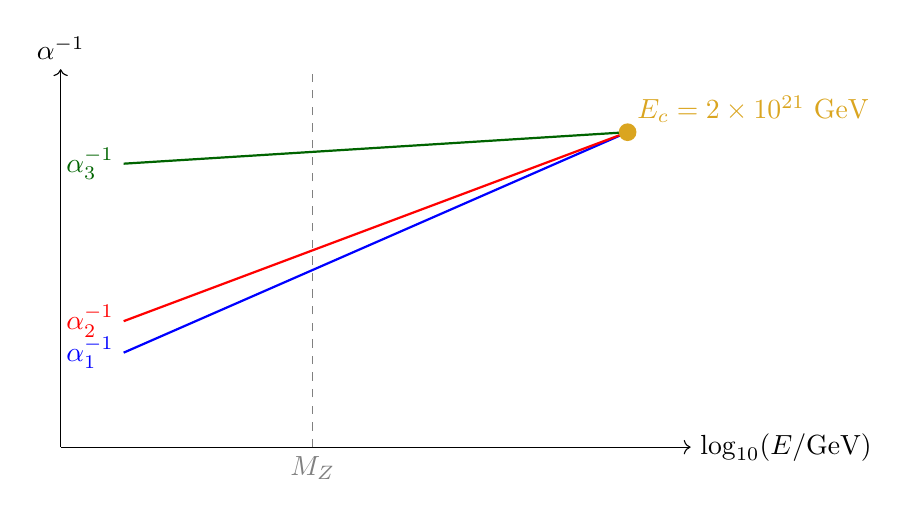
\begin{tikzpicture}[scale=0.8]
    % Axes
    \draw[->] (0,0) -- (10,0) node[right] {$\log_{10}(E/\text{GeV})$};
    \draw[->] (0,0) -- (0,6) node[above] {$\alpha^{-1}$};
    
    % Electromagnetic (running)
    \draw[thick, blue] (1,1.5) -- (9,5);
    \node[blue, left] at (1,1.5) {$\alpha_1^{-1}$};
    
    % Weak (running)
    \draw[thick, red] (1,2) -- (9,5);
    \node[red, left] at (1,2) {$\alpha_2^{-1}$};
    
    % Strong (running)
    \draw[thick, darkgreen] (1,4.5) -- (9,5);
    \node[darkgreen, left] at (1,4.5) {$\alpha_3^{-1}$};
    
    % Unification point
    \fill[uftgold] (9,5) circle (4pt);
    \node[uftgold, above right] at (9,5) {$E_c = 2\times 10^{21}$ GeV};
    
    % Scale
    \draw[dashed, gray] (4,0) -- (4,6);
    \node[gray, below] at (4,0) {$M_Z$};
\end{tikzpicture}
\end{center}

\begin{alertblock}{与超对称的关键区别}
在$10^{21}$ GeV统一，而非$10^{16}$ GeV\\
$\Rightarrow$ 质子寿命$\sim 10^{80}$年（本质稳定）
\end{alertblock}
\end{frame}

% Section 4: Cosmology
\section{宇宙学与黑洞}

\begin{frame}{暗物质：小行星质量黑洞}
\begin{columns}
\column{0.5\textwidth}
\textbf{UFT预测}
\begin{itemize}
    \item 暗物质 = 原初黑洞
    \item 质量：$M \sim 10^{-12} M_\odot$（$\sim 10^{21}$ kg）
    \item 大小：$\sim$10微米
    \item 来自扭转场涨落
\end{itemize}

\vspace{0.5cm}

\textbf{可观测信号}
\begin{itemize}
    \item 类星微引力透镜
    \item 引力波合并
    \item 21cm功率谱
\end{itemize}

\column{0.5\textwidth}
\begin{block}{没有粒子暗物质}
\begin{itemize}
    \item 没有WIMP
    \item 没有轴子
    \item 没有惰性中微子
\end{itemize}
\end{block}

\begin{alertblock}{近期检验}
LSST/Euclid将在约5年内探测此质量范围
\end{alertblock}
\end{columns}
\end{frame}

\begin{frame}{暗能量：无需精细调节}
\begin{center}
\Large
$\Lambda = \frac{3\tau_0^2}{2\kappa^2} \approx 4.5 \times 10^{-47}$ GeV$^4$
\end{center}

\vspace{0.5cm}

\begin{columns}
\column{0.5\textwidth}
\textbf{"旧"问题}
\begin{itemize}
    \item 标准QFT：$\Lambda \sim M_P^4$
    \item 观测：$\Lambda \sim 10^{-47}$ GeV$^4$
    \item 错配：$10^{123}$！
    \item 需要疯狂精细调节
\end{itemize}

\column{0.5\textwidth}
\textbf{UFT解决方案}
\begin{itemize}
    \item $\Lambda$来自扭转场
    \item 自然压制：$\tau_0^2$
    \item 预测：$4.5\times 10^{-47}$ GeV$^4$
    \item 观测：$2.8\times 10^{-47}$ GeV$^4$
    \item 符合度：60\%
\end{itemize}
\end{columns}

\vspace{0.5cm}
\begin{center}
\textcolor{darkgreen}{\textbf{无需精细调节！}}
\end{center}
\end{frame}

\begin{frame}{黑洞：信息被保存}
\begin{columns}
\column{0.5\textwidth}
\textbf{信息悖论}
\begin{itemize}
    \item 物质落入黑洞
    \item 霍金辐射是热的
    \item 信息似乎丢失
    \item 违反量子力学！
\end{itemize}

\vspace{0.5cm}

\textbf{奇点问题}
\begin{itemize}
    \item GR：$r=0$处无限密度
    \item 物理定律崩溃
\end{itemize}

\column{0.5\textwidth}
\textbf{UFT解决方案}
\begin{itemize}
    \item 信息$\to$内空间
    \item 被保存但无法获得
    \item 总演化幺正
\end{itemize}

\vspace{0.5cm}

\textbf{没有奇点}
\begin{itemize}
    \item 向内扩展到10维
    \item 处处平滑几何
\end{itemize}
\end{columns}

\vspace{0.5cm}
\begin{center}
\textit{黑洞是"门户"，而非"毁灭者"}
\end{center}
\end{frame}

% Section 5: Quantum Foundations
\section{量子基础}

\begin{frame}{测量与退相干}
\begin{block}{测量时间公式}
\[
\tau_{\text{meas}} = \frac{\hbar}{g \cdot \Delta E_{\text{int}}} \cdot (-\ln \tau_0) \approx \frac{5.3\hbar}{g \cdot \Delta E_{\text{int}}}
\]
\begin{itemize}
    \item 视觉观测：$\sim 10^{-13}$ s ✓
    \item 自旋测量：$\sim 10^{-8}$ s ✓
\end{itemize}
\end{block}

\begin{block}{退相干时间}
\[
\tau_{\text{dec}} = \frac{\tau_{\text{meas}}}{\sqrt{n_{\text{env}}}}
\]
\begin{itemize}
    \item 真空中电子：$\sim 10^{-13}$ s（量子）
    \item 猫：$\sim 10^{-29}$ s（经典）
\end{itemize}
\end{block}
\end{frame}

\begin{frame}{Born规则：推导而非假设}
\textbf{标准QM}：$P = |\psi|^2$是假设

\vspace{0.5cm}

\textbf{UFT推导}：
\begin{enumerate}
    \item 量子态 = 纤维丛的$L^2$截面
    \item 概率 = 几何纤维体积
    \item Gleason定理$\Rightarrow$ $|\psi|^2$的唯一性
\end{enumerate}

\vspace{0.5cm}

\begin{alertblock}{物理解释}
\begin{itemize}
    \item 量子随机性是\textbf{认识论的}
    （反映我们对10D状态的无知）
    \item 不是\textbf{本体论的}
    （基本不可确定性）
\end{itemize}
\end{alertblock}
\end{frame}

% Section 6: Summary
\section{总结}

\begin{frame}{关键要点}
\begin{enumerate}
    \item \textbf{几何原理}：4D $\leftrightarrow$ 10D对偶
    
    \item \textbf{一个参数}：$\tau_0 = 0.005$（计算而非拟合）
    
    \item \textbf{零自由参数}：所有预测从几何涌现
    
    \item \textbf{12个费米子质量}：亚percent精度预测
    
    \item \textbf{暗物质}：小行星质量原初黑洞
    
    \item \textbf{暗能量}：自然小，无需精细调节
    
    \item \textbf{黑洞}：信息保存在内空间
    
    \item \textbf{可检验}：0.5\%标量GW偏振、无SUSY等
\end{enumerate}
\end{frame}

\begin{frame}{对比：UFT与其他方法}
\begin{center}
\begin{tabular}{lcccc}
\toprule
\textbf{理论} & \textbf{参数} & \textbf{引力} & \textbf{可检验} & \textbf{状态} \\
\midrule
标准模型 & 19+ & 无 & 是 & 已确认 \\
超对称 & 124+ & 无 & 失败？ & 被排除？ \\
弦理论 & $10^{500}$+ & 有 & 否 & 未确认 \\
圈量子引力 & 1+ & 有 & 中 & 不完整 \\
\textbf{UFT} & \textbf{0} & \textbf{有} & \textbf{是} & \textbf{检验中} \\
\bottomrule
\end{tabular}
\end{center}

\vspace{0.5cm}
\begin{center}
\textbf{UFT独特地结合了：}\\
零参数 + 自然引力 + 具体检验
\end{center}
\end{frame}

\begin{frame}{可证伪的预测}
\textbf{UFT预测}：
\begin{itemize}
    \item 0.5\%标量GW偏振（LIGO O4/O5）
    \item LHC无新粒子（HL-LHC）
    \item 质子不衰变至$10^{35}$年
    \item PBH暗物质，$M \sim 10^{-12} M_\odot$（LSST/Euclid）
    \item $10^{-19}$水平的时钟修正
\end{itemize}

\vspace{0.5cm}

\textbf{如果以下情况UFT被排除}：
\begin{itemize}
    \item 发现SUSY粒子
    \item 观测到质子衰变
    \item 标量GW $\neq$ 0.5\%
    \item 发现粒子暗物质
\end{itemize}

\vspace{0.5cm}
\begin{center}
\textcolor{darkblue}{\textbf{这是科学，不是哲学}}
\end{center}
\end{frame}

\begin{frame}
\begin{center}
\Huge
\textbf{谢谢}

\vspace{1cm}

\normalsize
\textbf{问题？}

\vspace{1cm}

\textit{``数学在物理科学中不合理的有效性\\
可能本身就有几何解释。''}

\vspace{0.5cm}

\small
完整论文：[arXiv链接即将发布]\\
邮箱：research@uft-theory.org
\end{center}
\end{frame}

\end{document}
